\chapter{Plan de gouvernance des données}\label{chap:gouv}

\section{Conformité RGPD et conformité HDS}\label{sec:qualif}
\begin{table}[!htbp]\small
\caption{Qualification RGPD du traitement « entrepôt de pilotage »}\label{tab:qualif}
\begin{tabularx}{\linewidth}{@{}L{2.9cm}Y@{}}
\toprule\entete\textbf{Élément} & \textbf{Analyse}\\\midrule
Responsable & Selon la forme juridique du groupe CHU : directeur d'établissement public (CSP, art.~L.~6143-7), établissement support d'un GHT, ou responsables conjoints (RGPD, art.~26). DPO associé dès la conception (art.~25, 38). Sous-traitant : hébergeur certifié HDS (art.~28). \\
Finalité, base légale & Pilotage de l'activité, de la qualité et de la performance ; indicateurs agrégés ; pas de recherche. Art.~6.1.e et 9.2.h RGPD. \\
Formalités & Registre (art.~30) ; AIPD obligatoire (données de santé à grande échelle, art.~35.3.b). Conformité au référentiel CNIL des entrepôts de données de santé : déclaration de conformité envisagée. \\
Information, sources & Art.~13, 14 et 21 (livret d'accueil, affichage, opposition). S2 : noms publics, minimisés ; S3 : agrégats ; S4 : RGPD inapplicable aux défunts (considérant 27), noms écartés. \\
\bottomrule
\end{tabularx}
\end{table}

\textbf{Hébergement de données de santé (HDS).} La production exige un hébergeur certifié HDS (CSP, art.~L.~1111-8) pour les activités 1 à 4 et 6. Le référentiel HDS v2 est applicable depuis le 16 mai 2026. Le décret n°~2026-209 impose un stockage exclusivement dans l'UE/EEE et quinze mentions contractuelles (art.~R.~1111-11). Contre le risque extraterritorial : clés détenues par le CHU, option SecNumCloud si l'AIPD le demande. \textbf{La VM du bloc ne reçoit que des données de test} : elle n'est pas un hébergement de santé.

\section{Pseudonymisation, anonymisation et zones de sécurité}\label{sec:pseudo}

\textbf{Classification.} \textbf{C3} directement identifiant (Bronze S1 et séjours) : zone Z2, aucun accès humain nominatif. \textbf{C2} pseudonymisé (Silver, lignes Gold) : Z3, accès nominatif habilité et journalisé. \textbf{C1} agrégats sous secret statistique (vues \code{v\_ind\_*}) : Z4, RLS par profil. \textbf{C0} public (S2 hors noms, S3, S4 sans noms, COG, CIM-10) : intégrité et traçabilité.

\textbf{Pseudonymisation.} HMAC-SHA-256 avec clé de 256 bits, variable \emph{Password} lue par \code{tContextLoad} dans un fichier protégé. Pas de table de correspondance ; pseudonyme déterministe (suivi longitudinal) ; une clé par domaine ; rotation annuelle par recalcul complet.

\textbf{Anonymisation des agrégats (secret statistique).} Dans les vues \code{v\_ind\_*}, toute cellule de moins de \textbf{11 patients distincts} est masquée, seuil évalué après les filtres de lignes, avec masquage secondaire contre le calcul par différence (dans l'esprit du $k$-anonymat avec $k = 11$). Aucun identifiant ni pseudonyme n'est exposé dans les vues. Les résultats HAS, publics, ne sont pas concernés.

\begin{figure}[!htbp]\centering
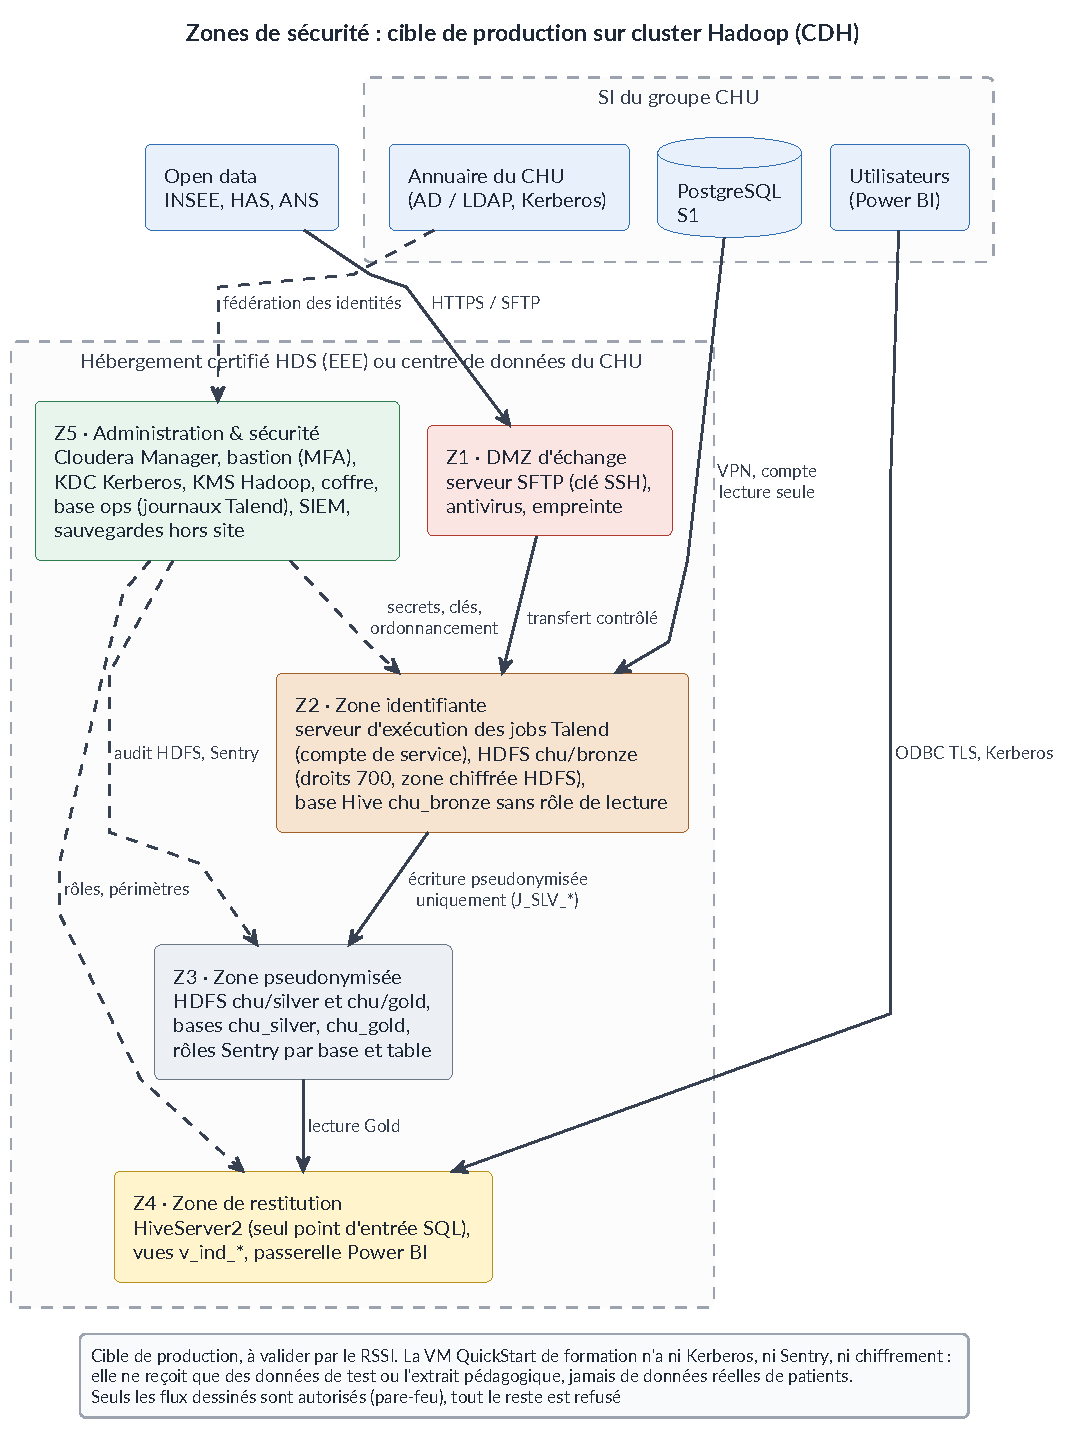
\includegraphics[width=\linewidth,height=0.5\textheight,keepaspectratio]{figures/16_zones_securite.pdf}
\caption{Zones de sécurité et flux autorisés (cible de production)}\label{fig:zones}
\end{figure}

\begin{figure}[!htbp]\centering
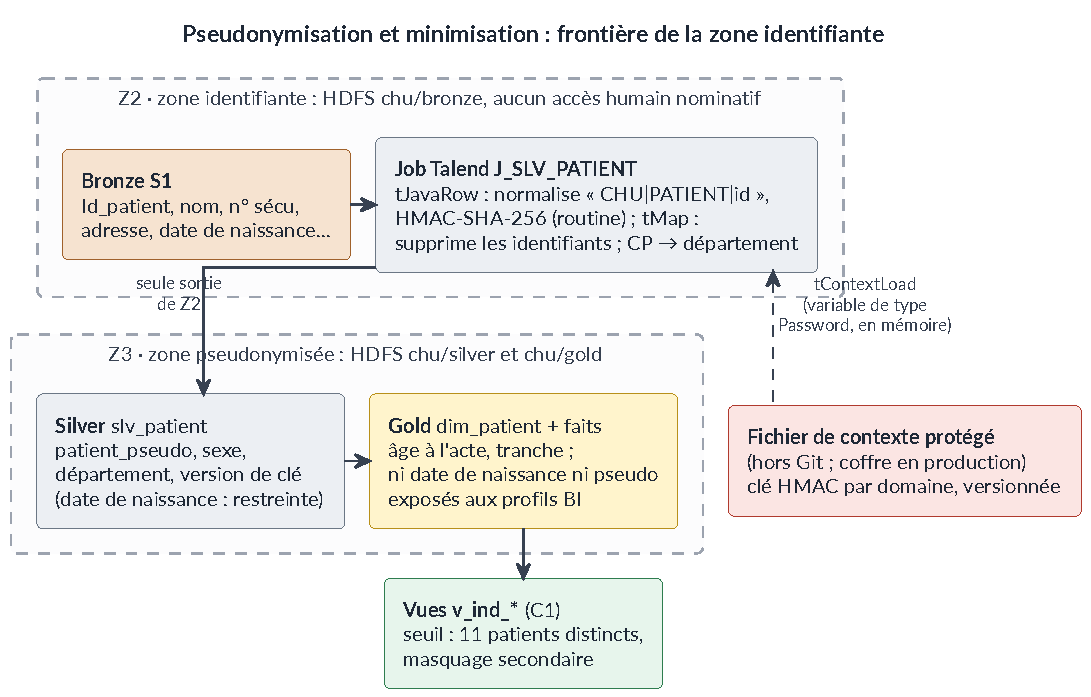
\includegraphics[width=\linewidth,height=0.3\textheight,keepaspectratio]{figures/15_pseudonymisation.pdf}
\caption{Chaîne de pseudonymisation (séparation de la clé et frontière de la zone identifiante)}\label{fig:pseudo}
\end{figure}

\section{Rôles et droits d'accès, traçabilité des flux}\label{sec:rbac}\label{sec:lignage}

\begin{table}[!htbp]\small\centering
\caption{Matrice RBAC (rôles $\times$ ressources)}\label{tab:rbac}
\setlength{\tabcolsep}{3.5pt}
\begin{tabularx}{\linewidth}{@{}Yccccccc@{}}
\toprule\entete
\textbf{Rôle} & \rotatebox{75}{\textbf{Bronze (C3)}} & \rotatebox{75}{\textbf{Silver (C2)}} & \rotatebox{75}{\textbf{Gold lignes (C2)}} & \rotatebox{75}{\textbf{Vues agrégées (C1)}} & \rotatebox{75}{\textbf{Rejets}} & \rotatebox{75}{\textbf{Journaux}} & \rotatebox{75}{\textbf{Export / SQL}}\\\midrule
Direction du groupe & & & & L & & & \\
Direction d'établissement & & & & F\textsubscript{étab} & & & \\
Praticien, chef de service & & & & F\textsubscript{prof} & & & \\
Analyste, DIM & & & L\textsuperscript{J} & L & & & oui\textsuperscript{J} \\
Data steward & & L\textsuperscript{J} & & L & L/E & & \\
Data engineer & & L\textsuperscript{T} & L\textsuperscript{T} & L & L & & \\
DPO, RSSI & & & & L & & L & \\
Jobs Talend (compte de service) & E/L & L/E & L/E & L/E & E & & \\
Power BI $\rightarrow$ HiveServer2 & & & & L & & & \\
Administrateur plateforme & & & & & & L & \\
\bottomrule
\end{tabularx}
\par\smallskip\raggedright\small Case vide : aucun accès ; L lecture ; E écriture ; F lecture filtrée par ligne (\textsubscript{étab} établissements de son périmètre, \textsubscript{prof} sa propre activité) ; \textsuperscript{J} nominatif, journalisé, sur demande justifiée ; \textsuperscript{T} temporaire, pour un incident.
\end{table}

\textbf{Principes} : moindre privilège, séparation des tâches, rôles par groupes de l'annuaire, recertification semestrielle. Trois niveaux de contrôle : (1) droits HDFS par couche ; (2) rôles Sentry, profils BI limités aux vues \code{v\_ind\_*} ; (3) sécurité au niveau des lignes de Power BI (RLS).

\textbf{Traçabilité des flux.} Flux : \code{ops.lot}, \code{ops.journal}, \code{ops.stat} (\code{tLogCatcher}, \code{tStatCatcher}, \code{tFlowMeterCatcher}), conservés 1 an. Lignage documenté (tableau~\ref{tab:jobs}) et porté par les données (\code{id\_lot}, \code{\_fichier\_source}, \code{\_ligne\_source}). Accès : journaux HiveServer2, audit HDFS, journal Power BI, 1 an au SIEM, revue mensuelle par le RSSI.

\section{Conservation, droits et incidents}\label{sec:retention}
\textbf{Conservation} : détail pseudonymisé Silver et Gold \textbf{10 ans glissants} ; agrégats anonymes sans limite après tests ; Bronze C3, rejets, répertoires de chargement : trois derniers chargements. \textbf{Droits} (art.~12 à 21 RGPD) : information patient ; accès et rectification sur le dossier source ; opposition et effacement par liste tenue en zone identifiante, appliquée au chargement suivant. \textbf{Incidents} : violation notifiée à la CNIL sous 72~h (art.~33), aux personnes si risque élevé (art.~34), à l'ARS et au CERT Santé.
